\input{../../Plantillas-Fomato/Tareas/tarea.tex}
\cabe{Geometría 3: Tarea 4}{Jhonny Lanzuisi, 1510759}
\usetikzlibrary{arrows}
\pgfplotsset{compat=1.16}
\begin{document}

	\tituloD{Geometría 3}{Cuarta Tarea}
	\subsection*{Ejercicio 1}
	
	\marginnote{
		\begin{minipage}{8cm}
			\begin{figure}[H]
				\begin{tikzpicture}
				\tkzInit[ymin=-0.5,ymax=3,xmin=-1,xmax=5]
				\tkzClip
				
				\tkzDefPoint(1,0){A}
				\tkzDefPoint(3,2){B}
				\tkzDefPoint(4,0){C}
				\tkzDefPoint(3.5,2.5){B'}
				\tkzDefPoint(4.5,0){C'}
				\tkzDefPoint(3,1){H}
				
				\tkzDefLine[perpendicular=through H](A,C) \tkzGetPoint{h}
				\tkzDefLine[perpendicular=through H](A,B) \tkzGetPoint{h'}
				
				\tkzLabelPoint[below left](A){$A$}
				\tkzLabelPoint[below right](C){$C$}
				\tkzLabelPoint[above left](B){$B$}
				\tkzLabelPoint[right](H){$H$}
				
				
				\tkzDrawSegment(A,B')
				\tkzDrawSegment(A,C')
				\tkzDrawPoints(A,B,C,H)
				\tkzDrawLine[add = 0.5 and -0.5](H,h)
				\tkzDrawLine[add = 0.55 and -0.5](H,h')
				\end{tikzpicture}\caption{Determinación de un triángulo dado un águlo y el ortocentro.}
			\end{figure}
		\end{minipage}
	}
	
	Sean $A$ el vértice de un ángulo agudo $\angle A$ y $H$ un punto interior a
	dicho ángulo. Determine el triángulo $ABC$ que tiene al punto $H$ como
	ortocentro.
	
	\begin{sol}
		Llamemos $c$ y $b$ a los lados del ángulo $\angle A$, consideremos las dos perpendiculares por $H$ a cada uno de estos lados y llamemos $B$ y $C$ a los puntos de intersección de dichas perpendiculares, distintos de los pies, con los lados $c$ y $b$ respectivamente. Entonces, por construcción, el triángulo $ABC$ es tal que sus alturas se intersectan en $H$, es decir, es el triángulo buscado.
	\end{sol}


\subsection*{Ejercicio 2}
Construir un triángulo conocido un vértice, el ortocentro y la circunferencia circunscrita.
	\marginnote{
	\begin{minipage}{8cm}hollla
		\begin{figure}[H]
			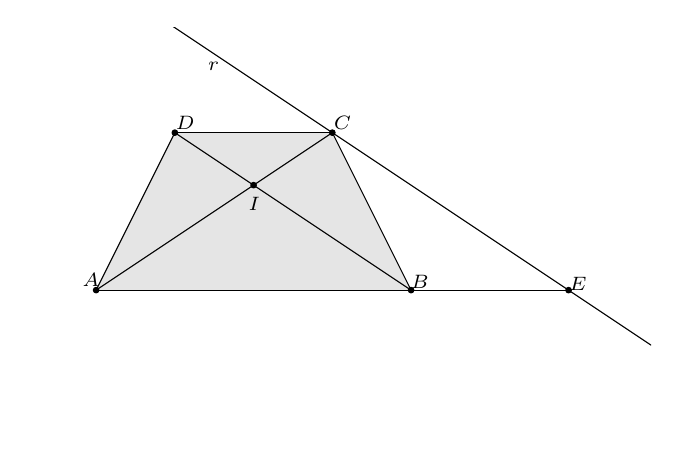
\begin{tikzpicture}[line cap=round,line join=round,>=triangle 45,x=1cm,y=1cm]

			\clip(-0.8690146553979121,-2.0018549308798055) rectangle (7.047515007813354,3.3331976682408246);

			\fill[line width=0.4pt,fill=black,fill opacity=0.10000000149011612] (0,0) -- (4,0) -- (3,2) -- (1,2) -- cycle;

			\draw [line width=0.4pt] (0,0)-- (4,0);

			\draw [line width=0.4pt] (4,0)-- (3,2);

			\draw [line width=0.4pt] (3,2)-- (1,2);

			\draw [line width=0.4pt] (1,2)-- (0,0);

			\draw [line width=0.4pt] (1,2)-- (4,0);

			\draw [line width=0.4pt] (3,2)-- (0,0);

			\draw [line width=0.4pt,domain=-0.8690146553979121:7.047515007813354] plot(\x,{(--12-2*\x)/3});

			\draw [line width=0.4pt] (4,0)-- (6,0);

			\begin{scriptsize}

			\draw [fill=black] (0,0) circle (1pt);

			\draw[color=black] (-0.06588845768082716,0.124790460013902) node {$A$};

			\draw [fill=black] (4,0) circle (1pt);

			\draw[color=black] (4.113645836561146,0.10840012944824721) node {$B$};

			\draw [fill=black] (3,2) circle (1pt);

			\draw[color=black] (3.1302260026218582,2.124410789023785) node {$C$};

			\draw [fill=black] (1,2) circle (1pt);

			\draw[color=black] (1.130605673611973,2.124410789023785) node {$D$};

			\draw [fill=black] (2,1.3333333333333333) circle (1pt);

			\draw[color=black] (2.0074883588745043,1.1000151286703612) node {$I$};

			\draw[color=black] (1.4911929460563782,2.8373901686297676) node {$r$};

			\draw [fill=black] (6,0) circle (1pt);

			\draw[color=black] (6.121461330853858,0.08381463359976506) node {$E$};

			\end{scriptsize}

			\end{tikzpicture}
		\end{figure}
	\end{minipage}
}
\begin{sol}
	Sean $A$ el vértice conocido, $H$ el ortocentro y $O$ el circuncentro (como se tiene la circunferencia circunscrita se puede determinar su centro) del triángulo buscado. Tomemos los puntos medios $A_h$ y $O_h$ de los segmentos $AH$ y $OH$ respectivamente. Entonces la circunferencia de centro en $O_h$ y que pasa por $A_h$ es la circunferencia de Feuerbach del triángulo buscado. Llamemos $D$ al punto de interseción (distinto de $A_h$) de la recta $A_hO_h$ con la circunferencia de Feuerbach, este punto $D$ es el punto medio del lado opuesto al vértice $A$ del triángulo buscado. Finalmente, tomemos la perpendicular a la recta $AH$ que pasa por $D$. 
	
	Entonces los dos puntos de intersección de dicha perpendicular con la circunferencia circunscrita son los otros dos vértices buscados. Nótese que, si el ortocentro se encuentra dentro, fuera, o sobre la circunferencia, el argumento anterior funciona igualmente.
\end{sol}
\begin{center}

\end{center}

\subsection*{Ejercicio 3}
Demostrar que las paralelas a dos lados de un triángulo por el baricentro
cortan al tercer lado en tres segmentos iguales.

\begin{sol}
	Sean $ABC$ un triángulo, $G$ su baricentro y $M_a$ el punto medio del lado opuesto al vértice $A$. Llamemos $A_g$ al punto medio del segmento $AG$. Como $AM_a$ es una mediana, la distancia $GM_a$ es la mitad de la distancia $AG$ y se sigue que los tres segmentos $AA_g$, $A_gG$ y $GM_a$ son congruentes. Si trazamos dos paralelas al lado $AB$ por los puntos $A_g$ y $G$ obtenemos que los puntos de corte $H$,$I$ de dichas paralelas con el lado $a$ dividen al segmento $BM_a$ en tres partes iguales puesto que esta es la construcción clásica para dividir un segmento en partes iguales. Lo mismo ocurre si trazamos dos paralelas al lado $AC$ por los puntos $A_g$ y $G$: obtendremos dos puntos de corte $J$,$K$ que dividen al segmento $M_aC$ en tres partes iguales. Por todo lo anterior, tenemos 
	\[ BI = \frac{2}{3} BM_a = \frac{2}{3} \frac{a}{2} = \frac{a}{3}, \]
	similarmente
	\[ CJ = \frac{2}{3} CM_a = \frac{2}{3} \frac{a}{2} = \frac{a}{3}, \]
	y por último
	\[ IJ = a-BI-CJ = a-\frac{a}{3}\frac{a}{3} = \frac{a}{3}. \]
	Y entonces los segmentos $BI,IJ$ y $JC$, que son los determinados por las paralelas a los lados $b$ y $c$ que pasan por $G$, dividen al lado $BC$ en tres partes iguales como se buscaba.
\end{sol}
%\begin{center}
%\begin{figure}[H]\centering
%	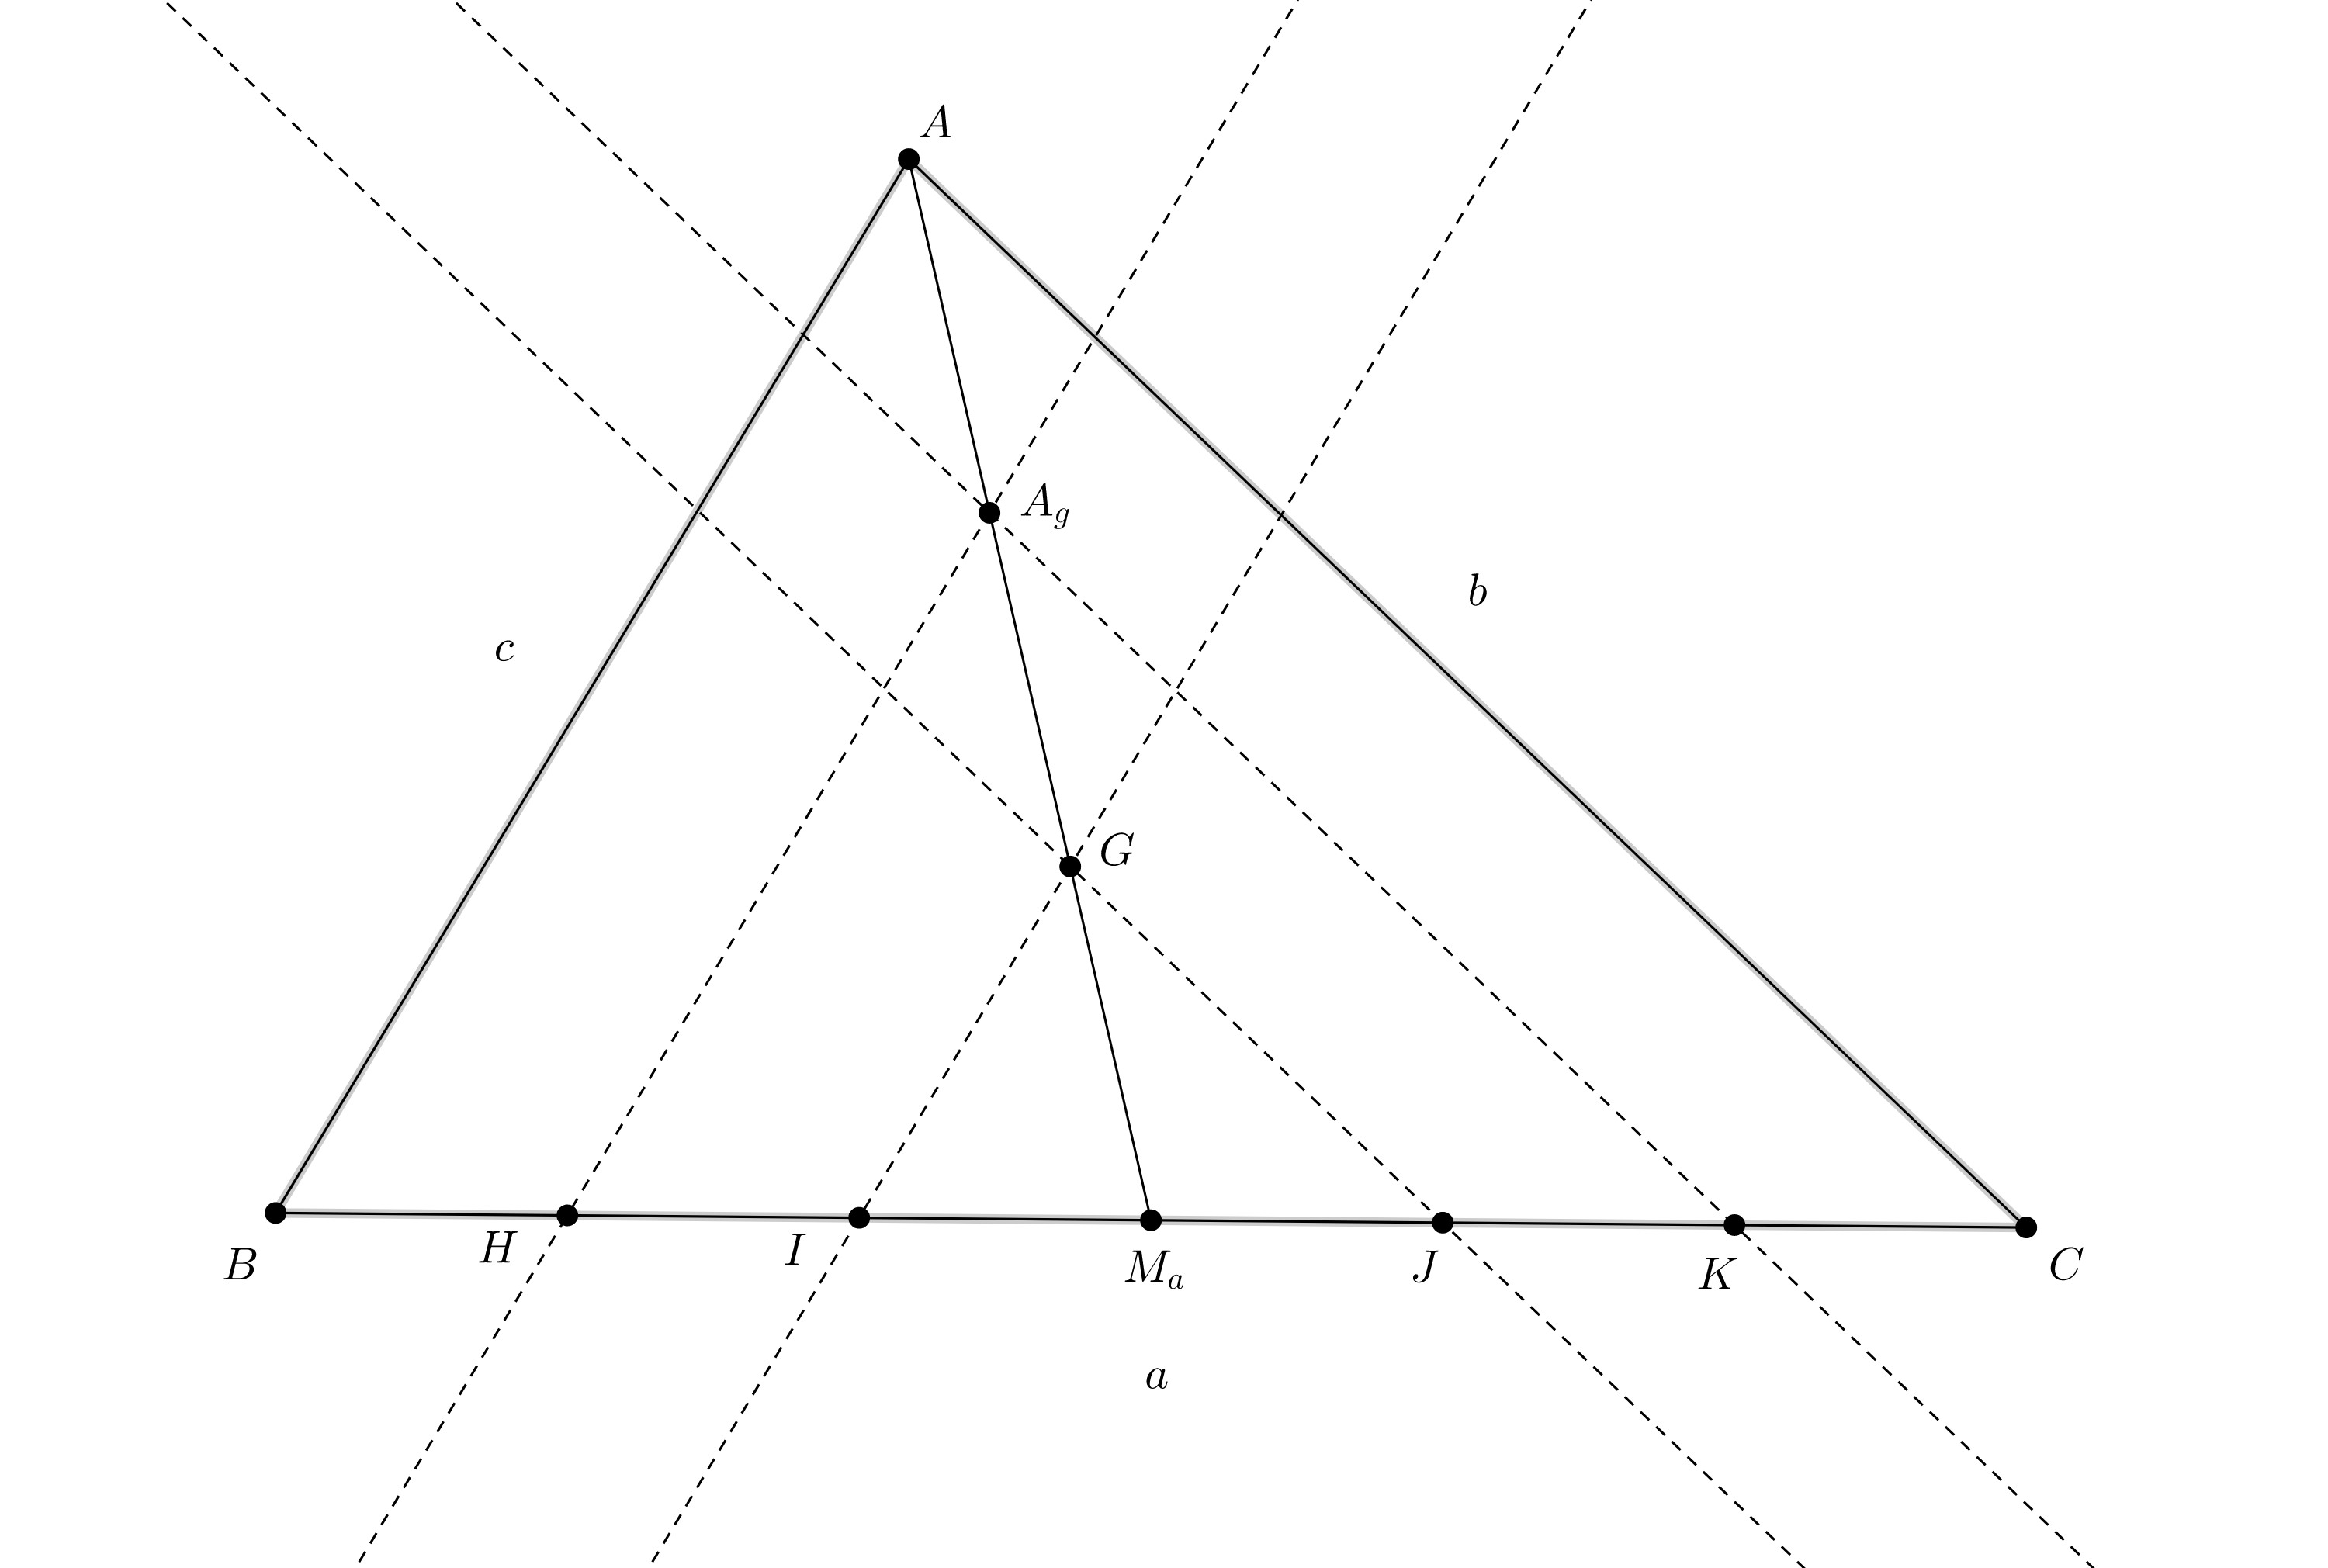
\includegraphics[width=1\linewidth]{pics/g5}
%\end{figure}
%\end{center}
\end{document}